\documentclass[a4paper]{article}

%%% packages %%%%%%%%%%%%%%%%%%%%%%%%%%%%%%%%%%%%%%%%%%%%%%%%%%%%%%%%%%%%%%%%%
\usepackage{graphicx}
\usepackage[utf8]{inputenc}
%\usepackage[T1]{fontenc}
\usepackage[ngerman]{babel}
\usepackage{subcaption}
\usepackage{amsmath,amssymb}
\usepackage{alltt}
\usepackage{natbib} % please use \citep and \citet instead of \cite
\usepackage{tikz}
\usetikzlibrary{positioning,automata}
\usetikzlibrary{shapes.geometric}
\usetikzlibrary{shapes.arrows}
\usepackage{array}
\usepackage{hyperref}
\usepackage{xcolor}
\usepackage{listings}
\usepackage[export]{adjustbox}
\definecolor{dark-red}{rgb}{0.4,0.15,0.15}
\definecolor{dark-blue}{rgb}{0.15,0.15,0.8}
\definecolor{medium-blue}{rgb}{0,0,0.5}
\hypersetup{
	colorlinks, linkcolor={dark-red},
	citecolor={dark-blue}, urlcolor={medium-blue}
}

\graphicspath{{./figs/}}
\DeclareGraphicsExtensions{.pdf}

\setlength{\parindent}{0mm}

\usepackage{fancyhdr}

%%% %%%%%%%%%%%%%%%%%%%%%%%%%%%%%%%%%%%%%%%%%%%%%%%%%%%%%%%%%%%%%%%%%%%%%%%%%

\makeatletter
\newcommand{\seminar}{Organic Computing (WS 2019/2020)}
\title{\textbf{Organic Computing:\\ Zusammenfassung}}\let\Title\@title
\newcommand{\sTitle}{Drahtlose Sensornetze}
\newcommand{\AuthorName}{Alexander Osiik}
\author{\AuthorName\\
	\href{mailto:alexander.osiik@student.uni-luebeck.de}{alexander.osiik@student.uni-luebeck.de}\\
	\small \seminar\\
	%    \small Service Robotics Group\\
	\small Institute of Computer Engineering, University of L\"ubeck\\
}\let\Author\@author
\makeatother

\pagestyle{fancy}
\renewcommand{\footrulewidth}{0.4pt}
\lfoot{\seminar}
\cfoot{}
\rfoot{\thepage}
\lhead{\AuthorName}
\rhead{\sTitle}

%%% %%%%%%%%%%%%%%%%%%%%%%%%%%%%%%%%%%%%%%%%%%%%%%%%%%%%%%%%%%%%%%%%%%%%%%%%%
\begin{document}
	\maketitle
\section{Einführung}
Computersysteme wrden immer komplexer. Die Netzwerke von kleinen, eingebetteten Systemen werden immer größer und komplexer. Es stellt sich die Frage, wie man unter solchen Bedingungen die Komplexität von
\begin{itemize}
	\item Design
	\item Implementierung
	\item Management
	\item Adaptation etc.
\end{itemize}
betrachtet und verbessert.\\
\\
In Organic Computing möchte man deswegen selbst \textbf{organisierte Systeme} entwickeln, die automatisch höherlevelige \textbf{Ziele} erfüllen und sich an die \textbf{Wünsche des Nutzers} anpassen. Dabei orientiert man sich oft an \textbf{lebenden Organismen}.
\subsection{Motivation}
Man möchte bei komplexen Systemen herausfinden, wie sie \textbf{funktionieren}, wie man sie \textbf{designed} und wie man sie \textbf{überwacht}.

\textbf{Moore'sches Postulat}
\begin{center}
	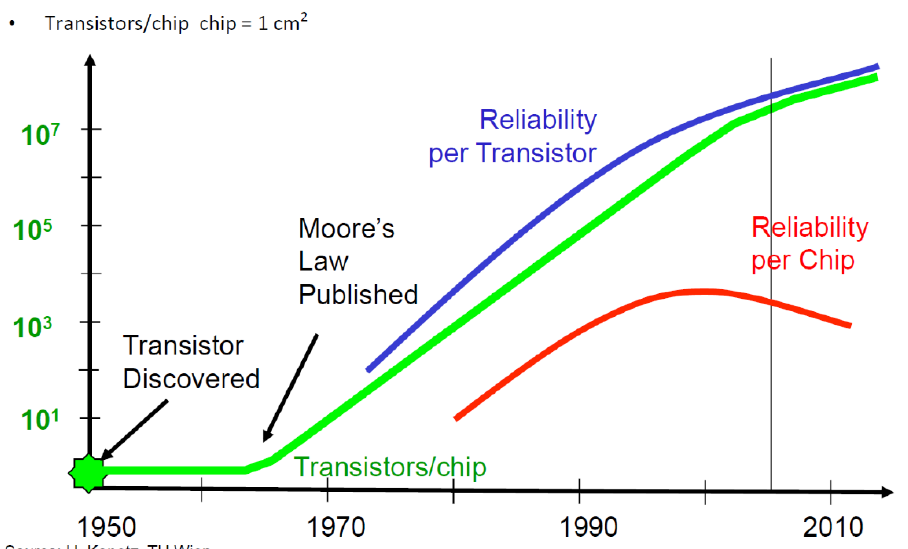
\includegraphics[height = 4cm]{Moore.png}
\end{center}
Bei komplexen Systemen wie autonomen Fahrzeugen stellen sich viele Fragen.
\begin{itemize}
	\item Wie \textbf{überwacht} man die Komplexität eines solchen Systems?
	\item Wie stellt man sicher, dass es keine \textbf{ungewollte Interaktion} zwischen zwei Systemen gibt?
	\item \textbf{WER} kontrolliert das Auto?
	\item Wer wird bei Fehlern zur \textbf{Rechenschaft} gezogen?
\end{itemize}
\textbf{Man möchte sich die Entwicklung komplexer Systeme dort abgucken, wo es schon erfolgreich war (zB. Gehirn).}\\

Komplexe Systeme entwickeln sich meistens durch \textbf{natürliche Selektion / Evolution}, oder durch tiefgründige \textbf{Forschung}, wo mehr und mehr komplexe selbst-organisierte Systeme gefunden werden können.
\subsection{Emergenz}
Unter Emergenz versteht man die spontane \textbf{Entwicklung von Systemcharakteristiken}, die sich durch Interaktion mehrerer Entitäten entwickeln. Diese emergenten Eigenschaften können nicht bei einer \textbf{isolierten} Entität erklärt werden.
\begin{itemize}
	\item Interaktion zwischen mehreren Entitäten
	\item \textbf{keine} zentrale Kontrollinstanz
	\item resultierende Patterns sind nicht vorher explizit programmiert 
\end{itemize}
Die Herausforderungen liegen darin, das emergente Verhalten \textbf{integrativ} zu verstehen (micro$\rightarrow$macro) oder das Verhalten individueller Elemente herauszufinden (macro$\rightarrow$micro).\\
\textbf{Beispiele:} Shockwave Traffic Jam, V-Formation Vögel\\

\subsection{Traditionelle Perspektive}
``Deterministic Centralized \textbf{(DC)} Mindset''
\begin{itemize}
	\item \textbf{D}: Relevanz von Randomisierung und Rauschen nicht berücksichtigt 
	\item \textbf{C}: Pattern wird durch Koordinator generiert
\end{itemize} 
\textbf{Eine falsche Annahme ist, dass bei systematischen oder systemweiten Effekte nur ein einziger Aktor betrachtet wird.}

\subsection{Organic Computing}
Bei Organic Computing betrachtet man das Zusammenspiel von (eingebetteten) Systemen mit bestimmten Eigenschaften, wie \textbf{viele Entitäten}, \textbf{Mobilität}, \textbf{Vernetzung} und spontane lokale Interaktionen \textbf{(Emergenz)}.\\

Was wir dafür brauchen sind viele, selbst-organisierte Entitäten, \textbf{robuste} Verhalten, flexible Verhalten, \textbf{Adaption} an dynamische Umweltfeatures und \textbf{Vertrauen} sowie \textbf{Kontrolle}. \\

\textbf{Kann man ein selbst-organisierenden und adaptierenden Mechanismus erstellen, ohne alle mögliche Zustände zu kennen?}
\subsubsection{Meta-Design}
\begin{itemize}
	\item Der Ingenieur macht Gesetze, kein Micromanagement
	\item Fuzzy-Platzierung statt rigide
	\item Adaptieren und selbst regulieren statt Kontrolle und Redesign
\end{itemize}
\subsection{Verhalten von Maschinen}
Das Verhalten von Maschinen ist ein kompliziertes wissenschaftliches Feld, sobald es genauso schwer zu verstehen ist wie ein biologisches System.
\subsubsection{Verhalten}
Verhalten ist, wie sich ein Lebewesen in bestimmten Situationen oder als Reaktion auf einen bestimmten Stimulus verhält.\\

Es gibt sozial geprägtes Verhalten, Verhaltenswissenschaften (Psychologie, Sozialwissenschaften, Neuralwissenschaften)
\subsubsection{Tierverhalten (Ethologie)} 	
Wissenschaftliche und objektive Forschung von Tierverhalten unter natürlichen Voraussetzungen. Verhalten wird als adaptives evolutionäres Extra behandelt.
\subsection{Komplexität und Opazität von Algorithmen}
Architektur und Training können sehr simpel sein, jedoch ist das Resultat sehr komplex, eher eine \textbf{black box}. Exakte funktionale Prozesse sind \textbf{hart zu interpretieren}, sogar von Wissenschaftlern, die diese Algorithmen erstellen! Sourcecode und Modell sind nur bedingt prädiktive Kraft.
\begin{center}
	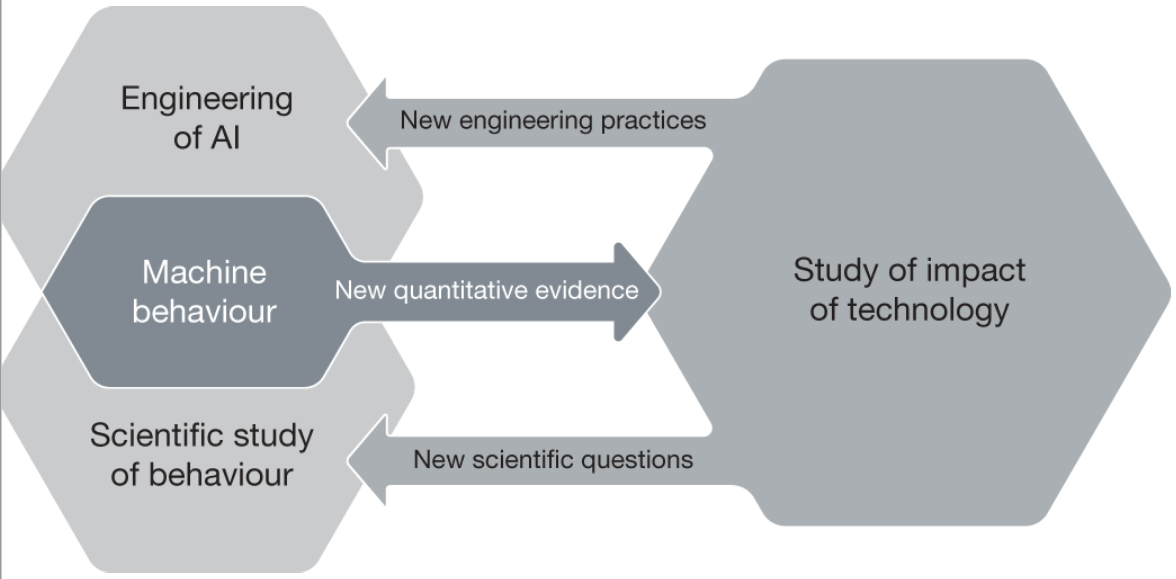
\includegraphics[height = 5cm]{AI.png}
\end{center}
Man soll zunächst \textbf{individuelles}, \textbf{kollektives} und dann \textbf{hybrides Mensch-Maschine} Verhalten studieren!
\newpage
\section{Von Bewegung zu Intelligenz}
Organic Computing ist Überwachung von komplexen technischen Systemen, und wie man diese Systeme \textbf{selbst-x}(adaptivm optimierend, reparierend etc.) macht. Man will also, dass diese System \textbf{intelligent} sind; sich in nicht antizipierten Situationen clever verhalten.\\
\textbf{Intelligente Entscheidungsfindung} ist das angemessene Verhalten in neuen Situationen, wobei man die Handlungsalternativen basierend auf den eigenen Präferenzen aussucht. \\
\\
Doch was ist die \textbf{Grundlage} der Intelligenz, und wie können wir sie \textbf{finden} oder \textbf{integrieren}?
\subsection{Wichtigkeit der Bewegung}
\textbf{Die Wahrnehmung der eigenen Bewegung und die anderer Entitäten ist Grundlage der Intelligenz.} Es ist eine wichtige Kompetenz, die über das Überleben in der Wildnis entscheidet. Was sich bewegt macht einen \textbf{lebendigen} Eindruck.\\
\subsubsection{Randomisierte Bewegung}
Die \textbf{randomisierte} Bewegung, bei der ein System sich in irregulärer Weise bewegt.
$$\sigma_s=\sqrt{\langle s_N^2 \rangle} = \sqrt{N} \ \ \text{Bewegung nach Münzwurfmodell} $$ 
Beim Random Walk wächst die Distanz zum Ursprung proportional mit der Zeit. Die unterliegende Wahrscheinlichkeitsdichte ähnelt der eines Diffusionsprozesses.\\
\textbf{Brown'sche Bewegung:} Zufällige Bewegung von Partikel in einer Flüssigkeit abhängig von Temperatur Bewegung.\\
\textbf{Drunkard's Walk:} Man startet eine Bewegung an Position $c_0$, jeder Schritt $c_i$ hat die \textbf{Länge L}. Nach $N$ Schritten ist die Distanz $\sqrt{N}L$ erreicht.\\
\textbf{Weitere Variationen:} Brown'sche Bewegung mit Drift:
$$\frac{\triangle x}{\triangle t} = \mu + \sigma\frac{\triangle W}{\triangle t}$$
\subsubsection{Ziel-orientierte Bewegung}
\textbf{Beispiel:} Bakterielle Chemotaxis\\
Hierbei haben Bakterien zwei Bewegungstypen:\\
 \textbf{Geradlinige Bewegung} (Rotation CCW), und \textbf{Taumeln}(Rotation CW). Der \textbf{Bias} ist hier die zeitliche Wahrnehmung, ob die Situation sich verbessert (weiterschwimmen) oder nicht (Taumeln). Die Modellierung erfolgt anhande von
 \begin{itemize}
 	\item Intrazellulären Modell
 	\item Zellulären Model
 	\item Populationsmodel (interzellulär)
 \end{itemize}
\subsection{Interaktion}
Es gibt grundsätzlich zwei Formen der Interaktion
\begin{itemize}
	\item Explizit: Es wird ein beabsichtigtes Signal gesendet
	\item Implizit: Physischer Kontakt, Kommunikation über die Umgebung
\end{itemize}
Die Signale können \textbf{Visuell}(Glühen, Farben), \textbf{Auditiv}(Heulen, Rufen), \textbf{Taktil}(Anfassen) und \textbf{Chemisch}(Pheromone, olfagorisches) sein\\

\ \ Bewegung nach Münzwurfmodell Kommunikation/Population braucht man denn? Wieviel Neuronen braucht man für Intelligenz? Wieviele Leute für eine gute Party?\\
\textbf{Beispiel:} Das Drei Körper Problem aus der Physik (Modellierung von 3 frei beweglichen abhängigen Partikeln)
\subsubsection{Simple Interaktion}
$N$ Partikel, die sich zufällig bewegen, Gruppen detektieren, stoppen, und eine gewisse Zeit warten. Wie aggregiert man alle $N$ Partikel in ein Cluster?\\
\textbf{Ansatz:} In großen Clustern länger bleiben.
\subsubsection{Kollaboration}
Bei zwei Agenten hat jeder die Wahl zwischen zwei möglichen Optionen:\\
 ``\textbf{Cooperate}'' oder ``\textbf{Defect}''\\
\begin{center}
	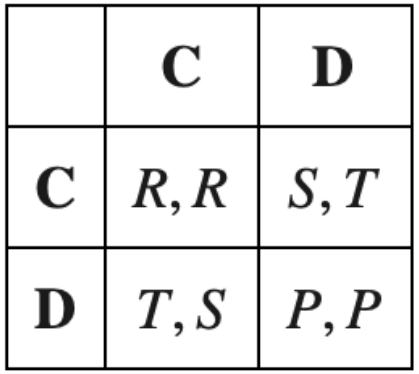
\includegraphics[height = 4cm]{PrisonersDilemma.png}
\end{center}

 Das \textbf{Iterated Prisoner's Dilemma} untersucht das obige Verhalten nach mehreren Runden. Hierbei ist die Frage, welche Strategie am schlausten ist (Keine Perfekte Information vorhanden, da Entscheidungsbaum simultan!):
 \begin{itemize}
 	\item Revenge!
 	\item Sofort Heimzahlen, aber 2.Chance geben
 	\item Immer Nett sein
 	\item Random
 \end{itemize}
\subsubsection{Evolution}
Idee: Wir benutzen künstliche Evolution für IPD um Strategien zu entwickeln und zu schauen, welche Strategie überlebt. Die getesteten Stratefien sind
\begin{itemize}
	\item Konditionale Kooperator
	\item betrügerische Überläufer
	\item Purer Überläufer
\end{itemize}
Man beobachtet jeweils eine zyklische Dominanz.
\subsubsection{Grün-Bart-Effekt}
Der Grün-Bart-Effekt ist ein Gedankenexperiment in verwendete Evolutionsbiologie selektiv zu erklären Altruismus unter den Individuen einer Spezies. Zwei sich erkennende Individuen benehmen sich \textbf{vetternwirtschaftlich}.\\

Dazu gehört
\begin{itemize}
	\item Fakultatives Helfen: Nur GB helfen
	\item Obligatorisches Helfen: Immer helfen, aber nur GB profitiert
	\item Fakultatives Schaden: Immer den $\neg$GB schaden
	\item Obligatorisches Schaden: Immer schaden, aber GB immun
\end{itemize}
\subsection{Emergente Taxis}
Kann ein Kollektiv von simplen Agenten zusammen etwas erreichen, was ein einzelner nicht schafft?\\
\textbf{taxis:} Bewegung als Antwort auf einen Stimulus\\
\\
Bei der \textbf{Emergent Phototaxis} möchte man
\begin{enumerate}
	\item Die Kollision mit anderen Robotern vermeiden
	\item Die Kohärenz beibehalten
	\item Roboter, die Kohärenz erlangen, bewegen sich random.
\end{enumerate}
Fazit: Es funktioniert!
\newpage

\section{Kollektive Intelligenz}
In Agentensystemen gibt es wenig bis \textbf{gar keine zentralisierte Kommunikation} oder Kontrolle. Es können nicht alle Agenten reden.\\

Exemplarische Design Probleme, die verteilte Computersysteme beinhalten, sind
\begin{itemize}
	\item Kontrollsystem für Routing in einem Netzwerk
	\item Routing in einem Stromnetz
	\item Verkehrskontrolle
\end{itemize}
\subsection{El Farol Bar}
Das El Farol Bar Problem ist ein Problem aus der Spieltheorie. Jeden Donnerstag wollen die Bewohner in die El Farol Bar. Die Bar ist klein, und niemand hat Spaß, wenn es zu voll ist.\\
Wenn weniger als $60\%$ gehen, haben alle mehr Spaß, als sie zu Hause gehabt hätten. Vice Versa.\\
\textbf{Problem:} Jeder entscheidet zur selben Zeit!
\subsection{Weisheit der Menschenmenge}
Idee: Man sammle Meinungen von einer Anzahl an Experten. Diese Meinungen werden verarbeitet (Mittel/Median). Die ``\textbf{kollektive}'' Lösung ist meistens \textbf{besser}, als die ``\textbf{individuelle}''.\\
\textbf{Francis Galton, Plymouth 1906}\\
\\
Die Effektivität der Weisheit wird oft auf das \textbf{Gesetz der Großen Zahlen} reduziert, bei dem der Durchschnitt eines statistischen Experiments den Erwartungswert $\mu$ erreicht, je mehr Versuche gemacht werden.\\
Hier ist es jedoch wichtig, dass die \textbf{Unabhängigkeit} jeder Wertung vorliegt, und Experten sich nicht gegenseitig beeinflussen. Das \textbf{Mitteln} reduziert zufällige Fehler, aber nicht \textbf{systematische Fehler}. 
\subsection{Kollektive Entscheidungsfindung}
\subsubsection{Best-Of-n Problem}
Man möchte aus $n$ Alternativen die beste finden.
\begin{itemize}
	\item jede Option hat die Qualität $\rho_i\in (0,1]$
	\item Mehrheit $M\geq (1-\delta)N$ wird gesucht, mit $0<\delta<<0.5$
\end{itemize}
\textbf{Wie lange} braucht der Prozess zum konvergieren?\\
\textbf{Wie oft} wird die Mehrheit erreicht?

\subsubsection{Ising Model}
Populäres Modell, welches aus dem Ferromagnetismus kommt. Jede Zelle eines Grids hat dabei die Zustände $s=\pm1$. Nachbarn wollen dabei im gleichen Zustand sein (Energieminimierung). Ein spontaner Wechsel ist abhängig vn der Temperatur möglich.
\begin{itemize}
	\item Magnetisierung $M=\sum_{i}s_i$
	\item Energie $E = \sum_{\langle ij \rangle}s_is_j$
\end{itemize}
Mit dem \textbf{Metropolis Algorithmus} wird pro Zeiteinheit ein Spin geflippt und geguckt, ob die Energie sich reduziert. Die Minimierung wird akzeptiert, wenn:
\begin{enumerate}
	\item $\triangle E \leq 0$: Exploitation mit WS = 1
	\item $\triangle E < 0$ : Exploration mit Wahrscheinlichkeit $A = \exp(-\beta\triangle E)$, $\beta = \frac{1}{T}$
\end{enumerate}
\subsubsection{Perkolation (Versickerung)}
Perkolation ist der Wasserfluss durch ein solides Substrat. \textbf{Perkolationstheorie} wird als Model für viele Szenarien verwendet, zb: Ausbreitung von \textbf{Epidemien}, \textbf{Waldbrände}, \textbf{Leitungsfähigkeit}...\\
Dabei beobachtet man ein interessantes, nicht-lineares Verhalten. Es gibt eine \textbf{kritische Wahrscheinlichkeit} $p^*$, wodurch ein kleines Cluster zu einem maximal großem Cluster mutiert.\\ \textbf{Beispiel:} Ein Feuer würde bis $p^*$ ausgehen, danach jedoch immer durchbrennen.\\

\begin{center}
	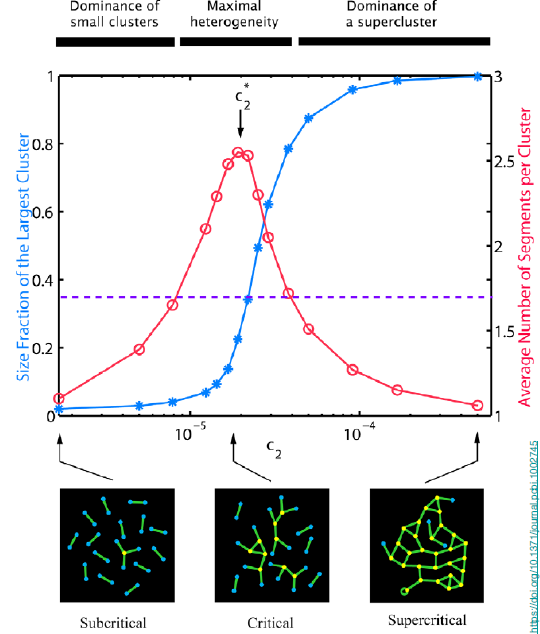
\includegraphics[height = 9cm]{Percolation.png}
\end{center}
\subsubsection{Individuelle Entscheidungsfindung}
Idee: Es gibt \textbf{Beweise} für eine der Alternativen, welche verarbeitet und \textbf{akkumuliert} werden bis eine \textbf{Schwelle} überschritten wird, nach der die \textbf{Entscheidung} getroffen wird.
\subsection{Geschwindigkeit vs. Genauigkeit}
Man kann schnell und ungenau sein, oder langsam und genau. Dies hängt nicht nur von Reaktionszeit ab!\\

Bei Kollektiven bekommt man meist Informationen durch seine Nachbarn. Beim \textbf{Ising-Modell} sind die Nachbarn fix, bei regulären Schwärmen bewegen sich die Nachbarn ständig! Die \textbf{lokale Stichprobe ist repräsentativ} für die gesamte Situation. 
\begin{itemize}
	\item Majority Rule (MR): Zähle die Meinungen der Nachbarn, bleib bei der Mehrheit (schneller)
	\item Voter Model (VM): Nimm einen zufälligen Nachbarn und übernimm seine Meinung (bei großen Schwärmen genauer)
\end{itemize}

\newpage
\section{Modellierung von OC-Systemen}
Start: Man möchte komplexe Systeme überwachen.
\begin{itemize}
	\item Was ist ein \textbf{System}?
	\item Was ist ein \textbf{komplexes System}?
	\item Wie können wir sie überwachen und \textbf{Performance} feststellen?
\end{itemize}
\subsection{Technische Begriffe}
\subsubsection{System}
Ein System ist eine Menge detaillierter Methoden, Prozeduren und Routinen, welche eine bestimmte \textbf{Aktivität} ausüben. Es ist eine organisierte \textbf{zweckgebundene Struktur}, die aus von einander abhängigen \textbf{Entitäten} abhängt. Diese Elemente beeinflussen sich gegenseitig und \textbf{erhalten die Existenz des Systems.}\\

Das \textbf{lineare System} ist dabei die simpelste Form eines Systems. Eine Änderung/Störung löst eine Antwort des Systems aus, welche proportional zur Eingabe ist.
$$y=Ax+B$$
Bei \textbf{nicht-lineare Systemen} ist die Systemantwort dementsprechend nicht proportional zur Eingabe, aber dennoch \textbf{vorhersehbar}. 
$$y = \sin x$$
\textbf{Nicht-lineare chaotische Systeme} scheinen unvorhersehbar zu sein, obwohl deren Systemgleichungen deterministisch sind. Ein solches System ist stark von den \textbf{Anfangsbedingungen} abhängig.
$$x_{n+1}=rx_n(1-x_n)$$
\subsubsection{Komplex vs Kompliziert}
Bei komplizierten Systemen ist die Lösungshierarchie \textbf{flach} (Evolution macht komplizierte Strukturen), während sie bei komplexen Systemen \textbf{vertikal}(Emergenz macht komplexe Strukturen) ist.
\subsubsection{Systemperspektive}
Betrachtung aller Verhalten des Systems als ein ganzes im Kontext seiner Umgebung ist die Systemperspektive. Bei der Systemperspektive soll das System bei weiterer Betrachtung nicht weiter reduziert werden.
\subsubsection{Komplexität}
Eigenschaft eines Systems, \textbf{alle} seine Eigenschaften nicht durch \textbf{einen} einzigen Formalismus adäquat beschreiben zu können.
\subsubsection{Modellierung}
Ein Modell ist eine vereinfachte Formalisierung der durch den Modellbauer verstandenen Welt (nicht zwingend realitätsgetreu). Für agenten-basierte Modelle modelliert man \textbf{Probleme}, \textbf{nicht Systeme}!\\

Beim \textbf{Top Down} Ansatz wird das System vom ganzen ins kleine modelliert. Voraussetzung dafür ist, dass das Verhalten bekannt ist, welches man reproduzieren möchte. Man braucht also ein gutes \textbf{Verständnis vom gesamten System} und wie die Komponenten \textbf{interagieren}.\\

Beim \textbf{Bottom Up} Ansatz wird das Verständnis vom System jedoch mehr gestärkt. Man versteht, wie relativ einfache Einheiten miteinander vernetzen, und wie ein \textbf{deterministischer Regelsatz} zur Entwicklung \textbf{komplexer Verhalten} führt.\\

Zu den agenten-basierten Ansätzen gehören \textbf{KI} (Agent ist autonome Einheit, welche Probleme löst), \textbf{Multi-Agenten Systeme} (Verteilte Kontrolle, kollektive Zielverfolgung) und \textbf{agenten-basierte Modellierung}. 

\subsection{Agenten}
Ein Agent ist ein \textbf{eingekapselter} Computer, welcher in einer Umgebung ausgesetzt ist. Er kann durch \textbf{flexible, autonome Aktionen} in dieser Umgebung ein vorgegebenes Ziel verfolgen.
\begin{center}
	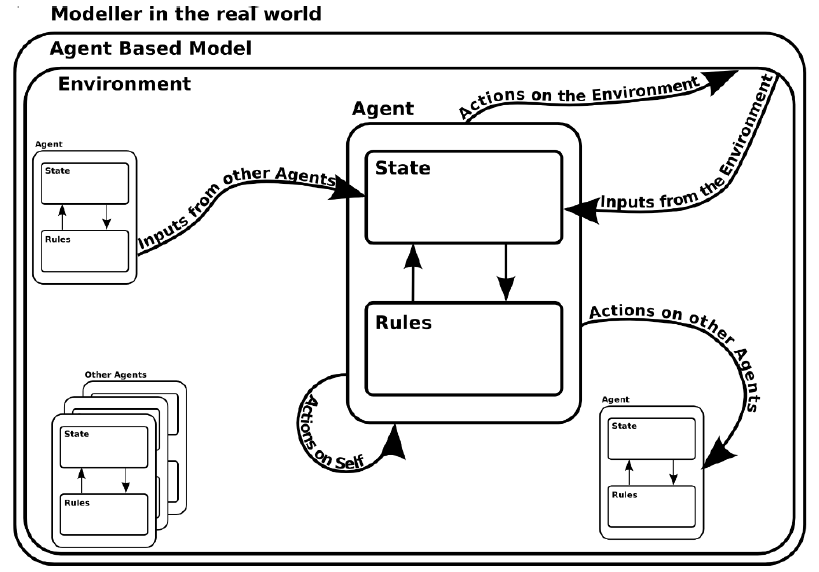
\includegraphics[height = 5cm]{Agent.png}
\end{center}
\subsubsection{Zustand / State}
Ein Zustand ist das Wissen über den Status der Umgebung. Dieses kann \textbf{öffentlich} oder \textbf{intern} sein. Zu jedem bestimmten Zeitpunkt ist der Zustand $s$ als Element der Zustandsmenge $S=\{s_1,s_2,\dots \}$ (Intern: $I=\{i_1,i_2,\dots \}$) vorgegeben.
\subsubsection{Regelnsatz}
Neben Zuständen verfügt der Agent über einen Regelsatz, welche die interne Beschreibung der Prozesse darstellt. Dies können zB  Transitionsregeln sein. Dabei gibt es die Varianten
\begin{itemize}
	\item regelbasiert
	\item abhängig von mehreren konkurrierenden Zielen
	\item Heuristiken
	\item Machine Learning
\end{itemize} 
\subsubsection{Aktion}
Eine Aktion hängt von anderen Agenten, internem Zustand (indirekte Umgebung) und dem Regelsatz ab. Eine Aktion beeinflusst dabei genau diese.
\subsubsection{Umgebung}
Eine Umgebung ist alles, was kein Agent ist, aber relevant für das Modell ist. Sie gibt \textbf{Informationen}, \textbf{Struktur} und \textbf{Stimuli}. Sie beeinflusst die Agenten, und wird von ihnen beeinflusst.
\subsubsection{Zeit}
Bei Agentensystemen betrachtet man in der Regel \textbf{diskrete Zeit}. Ein Zeitschritt ist dabei alles zwischen zwei Zeitpunkten, in diesem Zeitschritt funktioniert alles \textbf{simultan}. Agenten-basierte Systeme laufen \textbf{parallel} und \textbf{asynchron}, die Auswahl der Erstberechnungen muss also \textbf{randomisiert} erfolgen, um \textbf{Unabhängigkeit} zu schaffen.
\subsubsection{Agententypen}
\begin{itemize}
	\item \textbf{Agenten mit Wahrnehmung (Reflex Agenten):}\\
	Sensordaten sind Wahrnehmung, aus der der Zustand der Umgebung bestimmt wird. Danach erfolgt eine Aktion.
	\item \textbf{Agenten mit internen Zuständen:}\\
	Agent hat internes Gedächtnis um den Zustand des Systems zu speichern. Der neue Zustand ist vom alten Zustand abhängig und der Wahrnehmung. Abhängig von \textbf{neuem} Zustand wird dann die Aktion ausgeführt.
\end{itemize}

\subsection{Multi-Agenten-Systeme}
Eine Menge von Agenten die in der gleichen Umgebung koexistieren. Dadurch können Aufgaben auf mehrere Agenten \textbf{aufgeteilt} werden, um die \textbf{Systemperformance} zu erhöhen, oder es können \textbf{komplexe Probleme} gelöst werden, die eine einzelner Agent nicht lösen kann.\\

\textbf{Wie koordiniert man die Agenten durch Kommunikation und Interaktion?}\\

Wichtige Eigenschaften sind:
\begin{itemize}
	\item Die Agenten sind \textbf{autonom}
	\item Ihnen steht nur \textbf{lokale} Information zur Verfügung
	\item Das System ist \textbf{dezentralisiert}
	\item Zur Kollaboration und Koordination müssen Aktionen \textbf{geplant}, \textbf{mitgeteilt} und \textbf{verhandelt} werden.
\end{itemize}

\subsection{Koordinationsmechanismen}
Bei der \textbf{Korrelation} gibt es nur eine lose/zufällige Verbindung zwischen bestimmten Events. Es herrscht \textbf{keine Kausalität}.\\

\textbf{Koordination} ist eine Eigenschaft der Agentengruppe, die eine Aufgabe löst. Es ist ein \textbf{kausaler} Prozess, der aus Kommunikation der Agenten entsteht.
\subsubsection{Kommunikationstypen}
Die Kommunikation von Agenten kann durch \textbf{Kommunikationstopologie}(Zentral, Dezentral) und \textbf{Informationsfluss}(Direkt, Indirekt) kategorisiert werden.
\begin{itemize}
	\item \textbf{Topologie:}\\
	Zentral: kein Informationsfluss zwischen Slaves\\
	Dezentral: Peer2Peer
	\item \textbf{Informationsfluss:}\\
	Direkt: Agent zu Agent, ohne Umgebung zu berücksichtigen\\
	Indirket: Durch die Umgebung (Constraints durch Master)
\end{itemize}
\subsubsection{Typen von Koordinationsmechanismen}
\begin{itemize}
	\item \textbf{Markierung-basiert:} (Zeichen, Signal)\\
	Markierungen können von anderen Agenten observiert werden, andere Agenten können Tags beeinflussen oder hinzufügen (Vertrauen und Sicherheit)
	\item \textbf{Token-basiert:}(alles, was Agenten in einer Gruppe teilen können)\\
	Für jedes Token gibt es nur wenige Instanzen, Agenten mit Token haben \textbf{exklusiven} Zugriff. (Selbstschutz und Rollenverteilung)
	\item \textbf{Markt-basiert:} (Kaufen, Verkaufen)\\
	Agenten kommunizieren durch Transaktionen (Ressourcen Zuweisung)
\end{itemize}

\textbf{Beispiel:} Ameisen nutzen Pheromone zur Kommunikation. Pheromone ist die akkumulierte Erfahrung aller Ameisen. Diese ``Information'' kann \textbf{aggregiert} werden oder \textbf{verdampfen}. Jeder Agent kann auf die Information zugreifen und Information hinzufügen. \textbf{(Dezentralisiert, Indirekt, Markierung-basiert)}
\subsubsection{Self X (OC in anderen Ländern)}
\begin{itemize}
	\item \textbf{Self-Healing:} Das System kann sich von Fehlern erholen
	\item \textbf{Self-Protection:} Das System identifiziert und wehrt sich gegen Angriffe
	\item \textbf{Self-Optimizing:} Das System finden ein optimales Verhalten für ein Szenario
	\item \textbf{Self-Adaptive:} Das System passt sich an Veränderungen der Umwelt an
\end{itemize}
\newpage

\section{Architekturen}
Man möchte das komplexe System, was man beobachtet, auch \textbf{beeinflussen}. Man möchte damit auch sicherstellen, dass das System innerhalb der \textbf{gegebenen Parameter} operiert.
\subsection{Observer-Controller Architektur}
\subsubsection{System under Observation and Control (SuOC)}
\begin{center}
	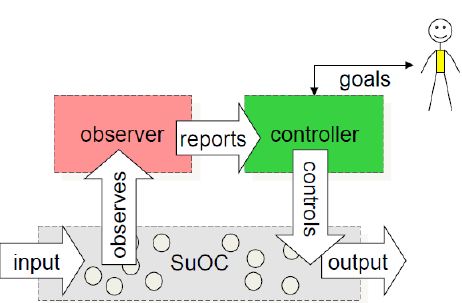
\includegraphics[height = 5cm]{SuOC.png}
\end{center}
\textbf{Start:} Ein einzelnes System, bestehend aus einer Gruppe von autonomen Robotern, welches als komplett bezeichnet werden kann. \\
\textbf{Input} sind alle Informationen (\textbf{Umgebungseffekte}), die ein SuOC zum reagieren braucht, aber nicht beeinflussen kann.\\
\textbf{Output} sind alle Informationen (\textbf{Parameter}) die vom SuOC bestimmt werden und von außen zugänglich sind.\\

Ein SuOC muss dabei folgende Anforderungen erfüllen:
\begin{itemize}
	\item \textbf{Ziele} erreichen und \textbf{Constraints} einhalten
	\item Verhalten von SuOC muss \textbf{beobachtbar} sein
	\item Performance muss \textbf{messbar} sein
	\item Muss \textbf{dynamische Kontrollfaktoren} besitzen
\end{itemize}

Der \textbf{Observer} (Beobachter) muss den aktuellen Systemzustand messen und evaluieren. Aus diesen Informationen muss er den nächsten Zustand vorhersagen können.\\


Der \textbf{Controller} ``überwacht'' den Prozess. Er \textbf{beeinflusst} das System so, dass die \textbf{Ziele erreicht} und die \textbf{Einschränkungen eingehalten} werden.\\
 Er unterbricht dabei \textbf{unerwünschtes emergentes} \textbf{Verhalten} und \textbf{rekonfiguriert} das System, um der Entwicklung von unerwünschtem Verhalten entgegenzuwirken. \\
 
 Möglichkeiten, das SuOC zu beeinflussen, sind:
 \begin{itemize}
 	\item Verhalten von Agenten ändern (\textbf{Regelsatz}) 
 	\item Das \textbf{Netzwerk} modifizieren um das Agentenverhalten zu ändern
 	\item Die \textbf{Anzahl} an Agenten(typen) erhöhen oder verringern
 	\item Die \textbf{Umgebung} modifizieren
 \end{itemize}
\subsubsection{Observer Modelle}
Der Controller kann dem Observer vorgeben, nach welchem \textbf{Observer-Modell} er handeln soll. Das Observer-Modell entscheidet darüber, welche \textbf{Features} überwacht werden solle, wie die \textbf{Daten analysiert} werden und wie der \textbf{zukünftige Zustand} vorhergesagt wird.
\subsubsection{Observer}
Der Aufbau des Observers ist wie folgt:
\begin{enumerate}
	\item \textbf{Monitor:} Überwachung der ausgewählten \textbf{Parameter} zu vorgegebener\textbf{ Sampling-Rate}. Diese werden in einem \textbf{Log-File} festgehalten, welche als \textbf{Basis für Vorhersagen} genutzt wird.
	\item \textbf{Pre-Prozessor:} Bereitet die Daten für das Verarbeiten vor (Filterung und Aggregation)
	\item \textbf{Data Analyzer:} Generiert den aktuellen Systemzustand (Parameter, entstehende Effekte). Die Methoden der Analyse hängen dabei vom gewählten Observer-Modell ab
	\item \textbf{Predictor:} Vorhersage des zukünftigen Systemzustands. Erlaubt dem Controller, Entscheidungen nicht nur abhängig von der Vergangenheit zu treffen. Dadurch wird die Reaktionszeit reduziert (Proaktives Verhalten)
	\item \textbf{Aggregator:} Kombiniert die oben genannten Daten zu ``\textbf{Situationsparametern}'', die dem Controller übergeben werden.
	
\end{enumerate}
\subsubsection{Controller}
Der Aufbau des Controllers ist wie folgt:
\begin{enumerate}
	\item \textbf{Mapping:} Implementiert Reaktion $A_i$ auf bestimmte Situationsparameter $C_i$. Erlaubt auch \textbf{erlernte Reaktionen} für unbekannte Situationen
	\item \textbf{Performance Evaluation:} Evaluation basiert auf Adaption von Selektoren. Abhängig davon wird das \textbf{Mapping} aktualisiert. \textbf{Online Learning} mit Historie von Aktions- und Situationsparametern
	\item \textbf{Simulation Model:} Erlaubt das generieren und evaluieren neuer Regeln. Diese werden durch Modifikation anderer Regeln oder Neuschöpfen hinzugefügt, nachdem sie in der \textbf{Simulation erfolgreich} waren (\textbf{Offline Learning}). Bietet dadurch mehr Systemsicherheit.
\end{enumerate}
Die Organisation kann dabei \textbf{zentral}, \textbf{dezentral} oder\textbf{ multi-level} erfolgen.
\subsubsection{Beispiel: Aufzugskontrolle}
Observer observiert en Bunching Effekt, Controller sorgt dafür, dass die Aufzüge äquidistant verlaufen. 
\subsection{Monitor-Analyze-Plan-Execute}
Historie: Problem bei IBM. Rechnersysteme werden komplexer und die Administration wird komplizierter. Man benötigt ein Paradigmenwechsel, um weniger Leute einstellen zu müssen und Kunden zufrieden zu machen.
\begin{center}
	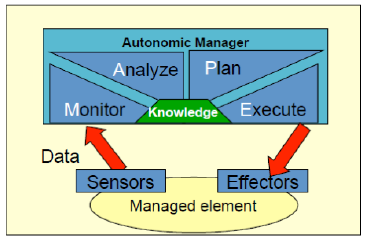
\includegraphics[height = 4cm]{MAPE.png}
\end{center}
\subsubsection{Autonomic Computing}
Computer, die sich \textbf{selbst verwalten} können, wenn ihnen ein \textbf{high-level Ziel} gegeben wird. Ähnlich dem menschlichen Nervensystem sollen auch Computern oder Verteilten Systemen \textbf{vitale Funktionen} zur Verfügung stehen.\\
Siehe auch: \textbf{Self-CHOP Prinzipien}
\subsubsection{Architektur}
\begin{itemize}
	\item \textbf{Autonome Systeme} sind ein Verbund von interagierenden autonomen Elementen
	\item \textbf{Autonome Elemente} besitzen Ressourcen und stellen Services zur Verfügung (für Nutzer oder andere AE). Sie interagieren mit anderen AE um Ziele zu erreichen. Sie haben einen oder mehrere zu verwaltende Elemente.
	\item Managed Elements (ähnlich wie SuOC) können ihren eigenen Kontrollzyklus haben. Beispiel hierfür wären Hardware- oder Softwareressourcen.
\end{itemize}
Der Autonome Manager ist für die Automation des IT Management Funktionalität verantwortlich. Er ist in der Regel für vier Aufgaben zuständig:
\begin{itemize}
	\item \textbf{Überwachen} von ME
	\item \textbf{Analyse} von Daten
	\item \textbf{Planen} von Aktionen
	\item \textbf{Ausführen} von Aktionen
\end{itemize}
\subsubsection{Monitor}
Automatische \textbf{Kollektion}, \textbf{Aggregation}, \textbf{Korrelation} und \textbf{Filterung} von Informationen über die Managed Ressource. Die Daten werden gesammelt, bis ein Symptom entdeckt wird. Die beobachteten Symptome werden zur Analyse weitergereicht.
\subsubsection{Analyse}
Zustäandig für Einhaltung von Beschränkungen. Observiert und analysiert Symptome, lernt Systemverhalten und sagt zukünftige Zustände voraus.
\subsubsection{Plan}
Generiert und wählt Prozeduren aus die die Managed Ressource beeinflussen. Generiert einen Plan der von GuideLines abhängt.
\subsubsection{Execute}
Zeitplanung und Ausführung der geforderten Systemänderungen. Kann mehrere oder einen einzigen \textbf{Managed Ressource} beeinflussen.
\subsubsection{Knowledge Source}
Repositorium für Symptome, Guidelines, Änderungsanfragen etc. Kann von vielen AM aus zugegriffen werden.
\subsection{Fazit}
\begin{itemize}
	\item ``Wissen'' ist über das O/C System verteilt
	\item MAPE: Sequenz von Operationen, O/C: Architekturkomponenten
	\item Bei O/C liegt der Fokus auf definierten Zielen
	\item MAPE hat keine expliziten \textbf{Offline Learning} Regeln
	\item Bei beiden gibt es keine Interaktion zwischen autonomen und organische Elementen
\end{itemize}	
\newpage

\section{Schwarm Intelligenz (ACO)}
	Wie kann man neue Mapping Regeln erstellen?\\
	Wie können wir die Auswahl an Mapping Regeln verbessern?\\
	$\implies$ Anpassung, Optimierung, Lernen
	
\subsection{Von Ameisen zu Algorithmen}
Rückblick: Ameisen Kolonie, Verhalten bei Binary Bridge Problem\\
\textbf{Erweiterung:} Ein Pfad ist doppelt so lang wie der andere. Im Endeffekt ist die Pheromon-Konzentration auf dem kürzeren Pfad höher. Der längere wird trotzdem ab und zu gewählt.\\
\subsubsection{Double Bridge Experiment}
\textbf{2. Erweiterung:} Der kurze Pfad wird erst später eingefügt. Die Ameisen vergessen jedoch nicht den langen Pfad, da die Pheromon-Konzentration dort höher ist.\\
Als Stochastisches Modell: $p_{is}(t)$ als Wahrscheinlichkeit, an Stelle $i$ den kürzeren Pfad zu nehmen.
$$p_{is}(t) = \dfrac{(\frac{1}{t_s}+\phi_{is}(t))^\alpha}{(\frac{1}{t_s}+\phi_{is}(t))^\alpha + (\frac{1}{t_l}+\phi_{il}(t))^\alpha}$$
Zeit für den kürzeren Pfad ist $t_s = \frac{l_s}{v}$\\
Pheromon-Konzentration auf kurzem und langem Pfad $\phi_{is}, \phi{il}$\\
$\alpha = 2$ experimentell bestimmt\\

Die Pheromonkonzentration wird bestimmt durch
$$\dfrac{d\phi_{is}}{dt}=\psi p_{js}(t-t_s)+\psi p_{is}(t) \ \ \ \ (i=1,j=2;i=2,j=1)$$
$$\dfrac{d\phi_{il}}{dt}=\psi p_{jl}(t-rt_s)+\psi p_{il}(t) \ \ \ \ (i=1,j=2;i=2,j=1)$$
\subsubsection{Double Bridge Experiment als diskretes Model}
$$p_{is}(t) = \dfrac{(+\phi_{is}(t))^\alpha}{(\phi_{is}(t))^\alpha + ({t_l}+\phi_{il}(t))^\alpha}$$
Update von Pheromonen-Konzentrationen:
$$\phi_{is}(t)=\phi_{is}(t-1)+p_{is}(t-1)\psi_i(t-1)+p_{js}(t-1)\psi_{j} (t-1)$$
$$\phi_{il}(t)=\phi_{il}(t-1)+p_{il}(t-1)\psi_i(t-1)+p_{jl}(t-r)\psi_{j} (t-r)$$
$$(i=1,j=2;i=2,j=1)$$
\subsubsection{Kürzeste Pfade in Graphen}
Ein Graph $G=(N,A)$ ist gegeben mit Menge der Knoten $N$ und Menge der unidirektionalen Kanten $A$. Es besteht das Risiko, dass ungewollte Zyklen entstehen, wenn Ameisen immer Pheromone ablegen. \\
Ein Ansatz ist, dass die Ameisen ihre Pheromone nur auf dem \textbf{Rückweg} ablegen (\textbf{unnatürlich}).\\

Noch eine Erweiterung wäre, den Ameisen eine \textbf{Erinnerung} an den\textbf{ bisherigen Pfad} und die entstandenen \textbf{Kosten} zu geben. Dadurch werden Zyklen detektiert. Die Menge der abgelegten Pheromone ist proportional zur Qualität der Lösung.

\subsubsection{Simple Ant Colony Algorithm}
Die Pfadwahl ist \textbf{probabilistisch} und hängt von der Pheromon-Konzentration ab. Auf dem Weg zum Ziel werden keine Pheromone abgelegt. Die Sequenz der \textbf{Wegpunkte} wird gespeichert. Durch \textbf{Backtracking} werden die Pheromone aktualisiert, die \textbf{Kosten} für den gefundenen Pfad werden berechnet und die \textbf{Evaporation} der Pheromone wird simuliert.\\

Die Pheromon-Konzentration $\tau_{ij}$ von $i$ zu $j$ ist initial $= 1$.\\
Die Wahrscheinlichkeit, dass die Ameise $k$ einen Pfad $i\rightarrow j$ wählt, wird berechnet als
$$p_{ij}^k = \left\{
\begin{matrix}
\dfrac{\tau_{ij}^\alpha}{\sum_{l \in N_i^k}\tau_{il}^\alpha}, \ \ \ \text{ if } j \in N_i^k\\\\
0, \ \ \ \ \ \ \ \ \text{ if } j\notin N_i^k
\end{matrix}
\right.$$
$N_i^k$ sind alle Knoten die von $i$ erreichbar sind.\\

Zyklen werden eliminiert, indem der Pfad nochmal durchsucht wird und Sequenzen zwischen zwei Zahlen eliminiert.\\
\\
Update der Pheromon-Konzentration durch ablegen (kann von Länge des Pfades abhängen)
$$\tau_{ij} \leftarrow \tau_{ij}+\triangle\tau^k$$ 
Evaporation der Pheromone dann durch
$$\tau_{ij} \leftarrow (1-p)\tau_{ij}$$ 

\subsubsection{Fazit}
Update basierend auf der Qualität der Lösung konvergiert zur optimalen Lösung. Für größere Werte $\alpha,p$ konvergiert S-ACO jedoch schneller auf sub-optimalen Lösungen.

 
\subsection{ACO Metaheuristik}
Eine Metaheuristik ist ein allgemein anwendbares, generisches, nicht vom Problem abhängendes Schema zur Entwicklung heuristischer Prozesse. Es ist eine allgemein anwendbare Heuristik, die (iterativ oder konstruktiv) problemspezifische Heuristiken zu vorteilhaften Bereichen des Suchraums führt.\\

Künstliche Ameisen generieren potentielle Lösungen, indem sie zufällig durch einen verbundenen Graphen $G_C=(C,L)$ laufen. \\
Die Knoten sind Komponenten, $G_C$ ist der Konstruktionsgraph, $L$ sind die Verbindungen.\\
Die Beschränkungen $\Omega$ sind Verhaltensregeln der Ameisen.\\
Für jede $c_i\in C$ und eine Verbindung $l_{ij}$ wird eine Pheromon-Konzentration $\tau_i$ gesetzt.\\
Hinzu kommt die Komponente $\eta$ für jedes $c_i$ und $l_{ij}$, welche die heuristische Information ist.\\
Die Ameise $k$ sucht den Graphen nach einer optimalen Lösung $s^*\in S^*$. \\
Darüber hinaus besitzt er die Memory $M^k$, die wichtig ist, um Beschränkungen zu erfüllen und die aktuelle Lösung zu evaluieren.\\
Es hat einen Anfangszustand und Endzustand, wobei der aktuelle Zustand $x_r=\langle x_{r-1},i \rangle$ ist.
\begin{lstlisting}
procedure ACOMetaheuristic
  ScheduleActivities
    ConstructAntSolutions
    UpdatePheromones
    DaemonActions % optional
  end-ScheduleActivities
 end-procedure
\end{lstlisting}
 
\subsection{Traveling Salesman Problem}
Ziel: Finde den kürzesten Pfad, der alle Städte verbindet (Funktion $f$). Jede Stadt kann nur ein mal besucht werden (Beschränkung $\Omega$). Eine Ameise wandert von Stadt zu Stadt, bis alle Städte durch sind. Die Entscheidung, in die Stadt $i$ zu gehen, hängt davon ab, ob man schon drin war, oder von der Anzahl der Pheromone.\\
\textbf{Formal:} Gewichteter Graph $G=(N,A)$, wobei $(i,j)\in A$ ein Gewicht $d_{ij}$ hat.
\subsubsection{Ant System Algorithmus}
\begin{lstlisting}
procedure ACOMetaheuristic
  set parameters, initialize pheromone trails
  while (termination condition not met) do
	ConstructAntSolutions
	UpdatePheromones  
end-procedure
\end{lstlisting}
\newpage

Folgendes Vorgehen:
\begin{enumerate}
	\item Setze alle Konzentrationen auf $\tau_0 = \frac{m}{C^{nn}}$
	\item in jedem Schritt bewegt sich die Ameise gemäß \textbf{random proportional rule}
	$$p_{ij}^k=\dfrac{[\tau_{ij}]^\alpha\cdot[\eta_{ij}]^\beta}{\sum_{l\in N_i^k} [\tau_{il}]^\alpha\cdot[\eta_{il}]^\beta}$$
	Als Heuristik wird der Abstand der Knoten gewählt 
	$$\eta = \frac{1}{d_{ij}}$$
	Hierbei $\alpha = 1$ und $\beta= 2-5$ ganz gut
	\item Update der Pheromone ist dann Evaporation
	$$\tau_{ij} \leftarrow (1-p)\tau_{ij}$$ 
	und erhöhte Konzentration (je nachdem wie oft der Pfad begangen wurde)
	$$\tau_{ij} \leftarrow \tau_{ij}+\sum_{k=1}^{m} \triangle \tau_{ij}^k$$ 
	Wobei $\triangle \tau_{ij}^k = \dfrac{1}{C^k}$, $C^k$ kosten der Tour
\end{enumerate}
\textbf{Weitere Optimierungen:}
\begin{itemize}
	\item 2 Exchange
	\item Mehr Fokus auf Ausnutzen der Erfahrung
	\item Pheromon-Konzentration für die Ameise mit der besten Tour Updaten.
	\item Pheromone früher evapoieren
\end{itemize} 

\subsection{Anwendungsbeispiele}
\subsubsection{Vehicle Routing Problem}
Es gibt ein Depot mit dem Index $0$. Es gibt $n$ Kunden, wobei jeder Kunde $i$ die Nachfrage $b_i$ nach dem selben Produkt hat. Es gibt mehrere Transportvehikel, alle haben Kapazität $B$. Es gibt verschiedene Kosten zwischen Knoten $d_{ij}$.\\

\subsubsection{VRP mit Zeitfenster}
Hierbei hat jeder Kunde noch ein vorgegebenes Zeitfenster. Dabei sind die Constraints hierarchisch, d.h. man minimiert lieber die Anzahl der Vehikel statt die Reisezeit.
	
\subsubsection{AntNet}
Best-Effort-Routing gesucht in IP Netzwerken. Dabei soll das Verhalten adaptiv zum aktuellen Datenverkehr reguliert werden.\\

Das Netzwerk ist charakterisiert durch
\begin{itemize}
	\item Bandbreite und Latenz von Links (Kanten)
	\item Router (Store-And-Forward, Buffer, Routing Lookup)
\end{itemize}
Der ACO kann hierbei wie folgt angewendet werden:
\begin{enumerate}
	\item Die Prozedur ist das Aussenden der Ameisen zu einer Destination. Die Ameise sucht Pfad mit minimalen Kosten, basierend auf der Heuristik des Routers und der Memory der Ameise.
	\item Die Modellierung erfolgt durch Graph $G_C$ von Routern. Jeder Router erhält eine Pheromone Matrix, die angibt, wie gut es ist von $i$ nach $d$ via $j$ zu gehen.
\end{enumerate}
Und so weiter.
\newpage

\section{Analyse von OC Systemen}
Wie kann man ein OC System/ SuOC verstehen?\\
Von wo kommen die kreativen Ideen?\\
Kann Wissenschaft automatisiert werden?
\subsection{Wissenschaftliche Bemühungen}
Herausforderungen bei Analyse von OC Systemen:
\begin{itemize}
	\item Systeme sind komplex und nicht-linear
	\item Es herrscht selbst-Organisation und viele Interaktionen
	\item Es ist schwer, alle Effekte zu antizipieren
\end{itemize}
$\implies$ Kreativität ist gefordert!\\

\subsubsection{Wie entdeckt man?}
Wie und woher kommen sie Ideen zu wissenschaftlichen Entdeckungen? Zufall? Gibt es einen Algorithmus dafür?\\

``Art of Thought''
\begin{enumerate}
	\item Preparation: Am Problem arbeiten
	\item Inkubation: Problem verinnerlichen
	\item Andeutung: Spüren, dass eine Lösung auf dem Weg ist
	\item Erleuchtung: Kreative Idee wird bewusst
	\item Verifizierung: Lösung wird geprüft
\end{enumerate}

\subsubsection{Hypothese}
Eine Hypothese ist eine gebildete Vermutung in der empirischen Wissenschaft. Sie ist \textbf{testbar}(Es gibt evtl. Gegenbeispiele, Plausibilität) oder \textbf{falsifizierbar}.\\

Was kommt zuerst: Hypothese oder Daten? Formuliert man die Hypothese, weil man Daten gesehen hat (\textbf{Induktion})? Sammle ich Daten weil ich eine Hypothese habe (\textbf{Deduktion})?

\subsubsection{Norwood Russell Hanson}
Norwood Russel Hanson war ein amerikanischer Philosoph. Seine wissenschaftliche Entdeckung war die Argumentation von Daten zu Hypothesen. Er entwickelte das \textbf{Hypothesis Catching}
\begin{enumerate}
	\item Fange eine Hypothese
	\item Teste sie
	\item Verfeinere oder Verwerfe
	\item Fang nochmal an!
\end{enumerate}
\textbf{Markov Ketten} können benutzt werden, um auf micro-level einen \textbf{individuellen Agenten} zu beschreiben oder auf macro-level das ganze\textbf{ SuOC }zu beschreiben.\\

Selbst-Organisation basiert auf 4 Komponenten:
\begin{itemize}
	\item positive und negative Rückkopplung
	\item Fluktuationen (zufällige Ereignisse)
	\item Mehrere Interaktionen
	\item Balance zwischen Exploitation und Exploration
\end{itemize}

Um nun OC Systeme zu analysieren, muss man zunächst \textbf{inkrementell} OC Systeme \textbf{modellieren}. Man sucht für das vorliegende System und Szenario ein \textbf{key feature} heraus, welches die relevanteste Eigenschaft des Systems ist. Danach versuchen wir, \textbf{Markov Zustände} $s\in S$ zu finden, die die Klasse der konfigurierten Zustände $C' \subset C$ repräsentiert. $S$ ist dann nach key-feature $s_f\in S_f$ strukturiert, $s \in S\backslash S_f$\\

Wir möchten also 
\begin{enumerate}
	\item eine Markov Kette erstellen,
	\item die Rückkopplung überprüfen
	\item verfeinern und dann mit 2. weitermachen, oder mit 1. von vorne starten
\end{enumerate}
\subsubsection{Key Feature Transitionen}
Eine \textbf{bool'sche Funktion} $f$ bestimmt, ob ein Agent $a$ das \textbf{key feature} hat. Die Teilmenge der Agenten mit key feature zur Zeit $t$ ist definiert durch
$$A_f(t)=\{a|f(a,t)\}$$
Die Verhältnis von Schlüsselmerkmalen $k$ errechnet sich durch
$$k=\dfrac{|A_f(t)|}{|A(t)|}$$
Wir sagen dann, dass $s_f\rightarrow s$ und $s\rightarrow s_f$ Key-Feature-Transitionen sind, weil sich dann das Schlüsselmerkmal mind. eines Agenten ändert mit Auswirkung auf das Gesamtsystem.\\
 Die Wahrscheinlichkeit für eine solche Transition mit einem Verhältnis $k$ ist
$$P_{s,s_f}(k)=\dfrac{P(s\rightarrow s_f,k)}{P(s\rightarrow s_f,k)+P(s_f\rightarrow s,k)}$$
Die Transitions-Wahrscheinlichkeit $P_{s,s_f}(k)$ kann auch \textbf{empirisch} gemessen werden und durch einen Octant analysiert werden: 
\begin{center}
	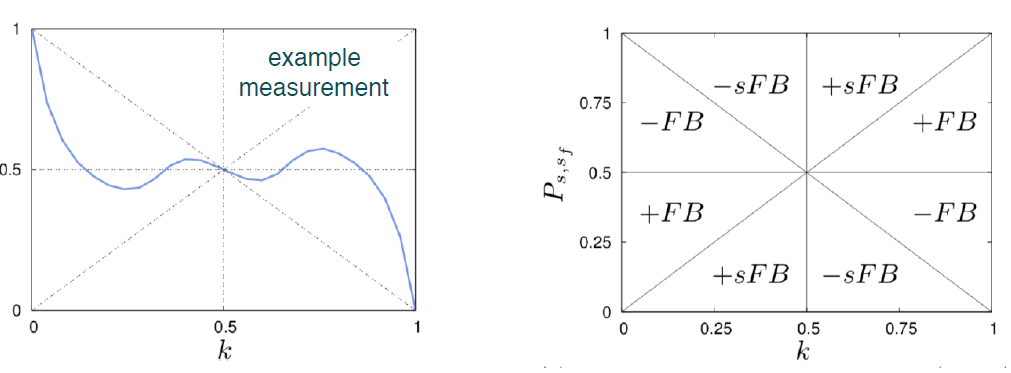
\includegraphics[height = 4cm]{TP.png}
\end{center}

\subsection{Exemplarische Analyse}	
Heuschrecken Bewegung\\
$$x_i(t+1) = x_i(t) + v_0 v_i(t)$$
$$u_i(t+1)=\left\{
\begin{matrix}
	G(L_i(t), R_i(t)),\text{ with probability }P_d\\
	-u_i(t), \text{ with probability }P_n\\
	u_i(t),\text{ else}
\end{matrix}
\right.$$

$$G(L,R)=\left\{
\begin{matrix}
-1, \ L>R\\
+1, \ R > L\\
u_r, \ R=L
\end{matrix}
\right.$$

\begin{center}
	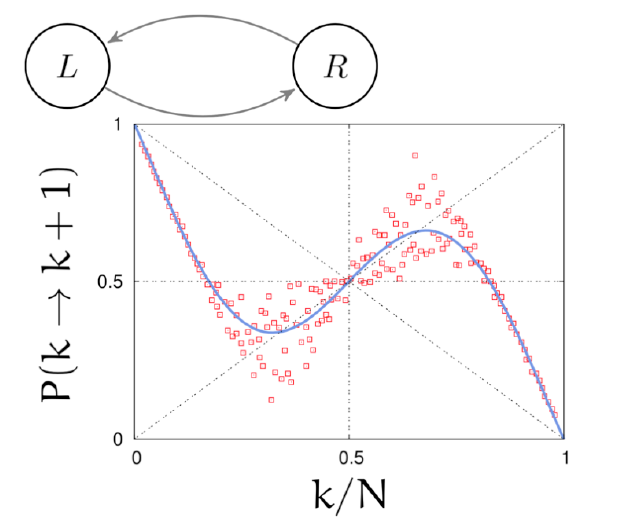
\includegraphics[height = 6cm]{LR.png}
\end{center}

\subsubsection{Interpretation}
Micro-lvel Markov Ketten reflektieren nicht alle relevanten Systemeigenschaften. Das Wechseln als eine Minorität führt echtes Feedback ein, kleine Komponenten zeigen Fluktuationen, die als negatives Feedback beitragen.
\newpage

\section{Robustheit und Vertrauen}
Woher wissen wir, ob das System \textbf{sicher} ist?\\
Wie verhält sich das System bei Fehlern und Störungen?\\
Wie Flexibel ist es?\\
Können wir dem System trauen?

\subsection{Robustheit}
Unter \textbf{Robustheit} versteht man die Fähigkeit eines Systems, auch im Falle von Parameterwechsel das gewünschte Verhalten zu garantieren. Die Funktion wird beibehalten, egal ob sich die \textbf{interne Struktur} ändert oder die \textbf{Umgebung}.\\

Ursachen für Störungen und Fehler sind in der Regel
\begin{itemize}
	\item ein falsches Systemmodell
	\item Numerische Fehler
	\item Varianz der Parameter
	\item oder einfach Abnutzung
\end{itemize}

Unter \textbf{Flexibilität} versteht man die Fähigkeit des Systems, sein Verhalten anzupassen, wenn sich Parameter oder Ziele ändern. 

\subsubsection{System Modell}
Ein System $S$ ist ein Tupel $S = (\mathcal{I},\mathcal{O},\beta)$
\begin{itemize}
	\item $\mathcal{I}$ ist das \textbf{Input} Interface: $$\mathcal{I} = R_s \cup C_c,$$ wobei $r \in R_s$ der rohe Sensor Input ist, und $c\in C_s$ der Control Input
	\item $\mathcal{O}$ ist das \textbf{Output} Interface. $o \in \mathcal{O}$ sind alle Parameter, die vom System beeinflusst werden.
	\item $\beta$ ist das \textbf{Verhalten}. Es definiert die Relation zwischen $R_s$ und $O_s$ zum Zeitpunkt $t$ und Antwort bei $t+1$. Es kann auch \textbf{zeitvariant} sein:
	$$\beta(t)\subseteq R_S \times O_s$$
	\item Dazu gibt es noch die Verhaltensspezifikation $\rho \subseteq R_s \times O_s$, welches die Performace Function ist. 
\end{itemize}
\subsubsection{Adaptivität}
Fähigkeit des Systems, sich an verschiedene Verhaltensspezifikationen $\rho$ anzupassen.\\
Das System ist \textbf{adaptiv} wenn es ein $t_1 \geq t_0$ gibt, sodass für alle $t$, $t_1\leq t \leq t_2$ gilt, dass $\rho(t)$ und $\beta(t)$ erfüllt sind.
\begin{center}
	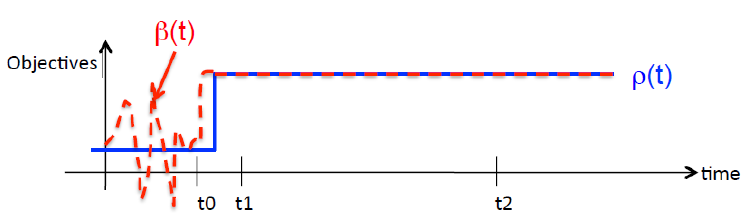
\includegraphics[height = 3cm]{rho.png}
\end{center}

Zur Evaluation erweitern wir das Systemmodell. Jedes System hat neben der Beschreibung $S=(\mathcal{I},\mathcal{O},\beta)$ auch den \textbf{aktuellen Zustand} $\mathbf{z}(t)$. Hinzu kommen die Parameter der \textbf{Umgebung} und die \textbf{interne Struktur} des Systems.\\

Zur Evaluation wird der Zustandsraum auf den Objective Space \textbf{gemappt}. Anhand der numerische Werte kann beurteilt werden, ob das System sich noch im Akzeptierten Zustandsraum befindet.

\subsubsection{Störung und unterteilter Zustandsraum}
Der Zustandsraum kann in 4 Zonen eingeteilt werden:
\begin{itemize}
	\item idealer Zustandsraum (Target Space TS)
	\item akzeptabler Zustandsraum (Acceptance State, AS)\\
	Zustände, die einen Evaluationswert innerhalb eines Grenzwerts haben
	\item Überlebenszustand (Survival State, SS)\\
	Das System kann von SS zu AS durch eine Kontrollsequenz noch zurückkehren
	\item Todeszone (Dead Space, DS)\\
	Kein zurück
\end{itemize}

Eine \textbf{Störung} $\delta$ kann intern oder extern vom System sein und führt zu einer Systemtransition von $\mathbf(t)$ zu $\delta(\mathbf{z}(t))$\\

Die Robustheit wird dann anhand der nichtleeren Menge $D=\{\delta_0, \delta_1,\dots  \}$ gemessen.\\
Es ist \textbf{stark robust} in Bezug auf $D$ wenn es für alle $\delta \in D$ im idealen Zustandsraum (TS) bleibt, sogar wenn sich Parameter ändern.\\
 Das System ist \textbf{schwach robust} in Bezug auf $D$ wenn es für alle $\delta \in D$ im akzeptablen Zustandsraum bleibt (AS)\\
 
 Ein System ist \textbf{adaptiv}, wenn es in Bezug auf $D$ ohne Fremdeinwirkung in AS zurückkehren kann. Es besitzt \textbf{Potenzial zur Adaptivität} wenn es nur mithilfe eines \textbf{externen Einflusses} zurückkehren kann.\\
 
\textbf{ Wichtig:}\\
\textbf{Flexibilität} bedeutet, dass ein System $S$ nach Änderung der \textbf{Spezifikation} oder Ziele zu AS zurückkehrt.\\
\textbf{Robustheit} bedeutet dass ein System $S$ nach einer \textbf{Störung} zu AS zurückkehrt.

\subsubsection{Arten von Unsicherheiten}
\begin{itemize}
	\item \textbf{Aleatorische Unsicherheiten} (=stochastische) durch \textbf{natürliche Variabilität} der Prozesse. Können nicht vom Menschen beeinflusst werden. Diese Unsicherheiten werden als Wahrscheinlichkeitsfunktion modelliert. Das benötigt jedoch eine Menge Daten, die oft nicht verfügbar ist.
	\item \textbf{Epistemische Unsicherheiten} (=subjektive) durch \textbf{unvollständiges Wissen} über den Prozess und die Modelle. Dazu gehören Unsicherheiten in
	\begin{itemize}
		\item Parameter: Input und Systemzustand
		\item Model: unvollständig oder falsch
		\item Szenario: relevantes Szenario, was nicht betrachtet wurde
		\item Numerik: Rundungsfehler
	\end{itemize}
\end{itemize}

\begin{center}
	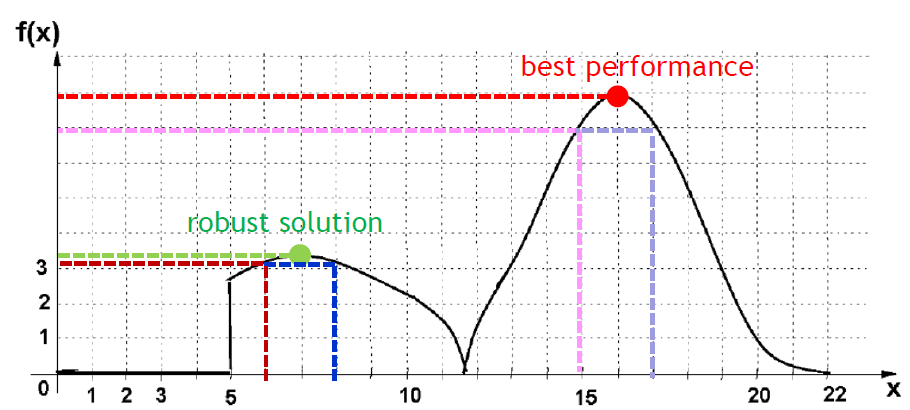
\includegraphics[height = 4cm]{RobustMax.png}
\end{center}

Um eine möglichst robuste Lösung zu bestimmen, versucht man das \textbf{minimal mögliche Resultat zu maximieren}. Dies ist vor allem für Probleme nützlich, wo eine \textbf{absolute Zuverlässigkeit} benötigt wird. Dabei gibt es einen Tradeoff zwischen \textbf{Qualität} und \textbf{Varianz} der Lösung.\\

Maximierung der erwarteten Performance:
$$f_{eff} = E(f(x+\delta)) = \int_{-\infty}^{+\infty}p(\delta)f(x+\delta)d\delta$$
Da $f$ oft unbekannt ist, schätzt man die Funktion mit \textbf{Monte-Carlo Estimation}, ``empirisch ermitteltes Mitteln'', ab. Ein Wert $x_0$ kann durch $n$ Samples $\hat{x}_i = x_0+\delta_i$ in der Nachbarschaft von $x_0$:
$$f_{eff}(x_0)=\dfrac{1}{n}\sum_{i=1}^{n}f(\hat{x}_i)$$
\subsubsection{Sampling}
\begin{itemize}
	\item \textbf{Zufällig}
	\item \textbf{Antithetisch:} $+\delta$ un $-\delta$, Mittelwert 0
	\item \textbf{Rasterbasiert:} Samples in kleinen Subgruppen, repräsentativ
	\item \textbf{Latin Hypercube Sampling:} Aufteilung in $k$ Teile, wobei jedes Teil nur von einem okkupiert wird
\end{itemize}

Ein Design ist \textbf{robust}, wenn die Varianz der Performance Function minimal ist.\\
Ein Design ist \textbf{zuverlässig}, wenn die Wahrscheinlichkeit von Systemversagen minimal ist.\\

\subsubsection{Zuverlässigkeit bestimmen}
\textbf{Reliability Based Design Optimization:}\\
Man möchte die Fitnessfunktion $f(\mathbf{x},\delta)$ so minimieren, sodass alle $J$ Constraints
$g_J(\mathbf{x},\delta)$ (Abstand zu \textit{infeasable space}) eingehalten werden (Linear Programming?):
$$min \ f(\mathbf{x},\delta)$$
$$\text{such that} \ Prob(g_k(\mathbf{x},\delta)\geq 0) \geq R_j, \ j\in\{1,2,\dots, J\}$$
$R_j$: W'keit dass Constraint $j$ erfüllt ist.\\

\textbf{Solution Based:}\\
Man generiere $n$ Lösungen $x+\delta$ und prüft für jede Lösung on $g_j(\mathbf{x},\delta)$ erfüllt. Misst man $r_j$ erfolgreiche Fälle, so kann man die $Prob-$Funktion zu
$$\dfrac{r_j}{n}\geq R_j$$
abschätzen. Natürlich muss man dabei nach Lösungen suchen, wo $R_J \not = 1$, um den Abstand zu minimieren.
Dabei ist das \textbf{globale} Optimum gar nicht so wichtig, da es in der Praxis weniger signifikant ist. Es wird nicht die \textbf{Sensibilität} des Systems betrachtet. 

\subsubsection{Robustheit - 2 Typen}
\begin{itemize}
	\item[\textbf{Typ 1:}] minimiert $f_{eff}$ in einer $\delta$-Nachbarschaft
	\item[\textbf{Typ 2:}] minimiert prozentuale Abweichung $|f_p(x)-f(x)\leq \eta|$: $f(x)$ soll besser sein als die gestörte Funktion $f_p(x)$ 
\end{itemize}
\subsubsection{Separated Consideration}
Neue Fitnessfunktion, die objective function und constraint violatoin trennt:
$$F(\mathbf{x})=\left\{\begin{matrix}
f(\mathbf{x}, \ \text{for} \ g_j(\mathbf{x})\geq0, \forall j\in\{1,2,\dots,J\}
)\\
f_{max} + \sum_{j=1}^{J} |g_j(\mathbf{x})|, \ \text{else}
\end{matrix}
\right.$$
\subsubsection{Pareto-Optimal und Paretodominanz}
Eine Lösung $x^*$ ist Pareto-Optimal, wenn es kein $\mathbf{x}\in S$ gibt, welches besser ist (Optimalität) und es in einer Dimension echt besser ist (?). Das $x$ muss also in einigen Dimensionen besser sein, aber im Schnitt schlechter abschneiden.

\subsection{Vertrauen}
``\textit{Vertrauen ist eine Wette mit bestimmten Risiko, nämlich dem, was mit durch Vertrauen gewonnen und verloren werden kann.}''\\

``\textit{Die Bereitschaft, sich für andere verwundbar zu machen, auf Grundlage der Erwartung, dass der Andere eine Aktion ausführt, die dem Vertrauensgeber wichtig ist.}''\\

Nutzer eines OC-Systems müssen Kontrolle aufgeben, da das System \textbf{selbst-organisiert} ist. Auch der Entwickler kann aufgrund der \textbf{Komplexität} des OC Systems keine klassischen Methoden anwenden. Im System selbst muss eine Einheit entscheiden, ob es einer anderen Einheit trauen kann.\\

\subsubsection{Aspekte von Vertrauen}
\begin{itemize}
	\item \textbf{Korrektheit:} Tut, was es soll. \textbf{Formale Methoden}
	\item \textbf{Sicherheit:} Autorisierter Zugriff. \textbf{Authentität}, \textbf{Autorisierung}, \textbf{Integrität}
	\item \textbf{Sicherheit:} Unerwartete Nebeneffekte. \textbf{Systemgrenzen}
	\item \textbf{Verfügbarkeit:} Verfügbar oder Erreichbar? \textbf{MTTF}, \textbf{MTTR}, \textbf{MTBF}
	\item \textbf{Robustheit:} Funktionalität unter verschiedenen Konditionen
	\item \textbf{Privatsphäre:} Nutzung privater Daten. \textbf{Persönliche Informationen}
	\item \textbf{Performance:} gewünschte Antwortzeiten
	\item \textbf{Glaubwürdigkeit:} Kommunkation mit Nutzer transparent? \textbf{Falsche Agenten}
	\item \textbf{Nutzbarkeit:} User Interface?
\end{itemize}
\subsubsection{Wie misst man Vertrauen?}
In verteilten OC Systemen wird Vertrauen auf die Verfügbarkeit reduziert, die von anderen Knoten observiert werden kann.\\

Dafür verwendbare Metriken wären die Anzahl der angekommenen \textbf{Delayed ACK}:
\begin{itemize}
	\item Mittel: $\dfrac{\sum_{i=1}^{n}x_i}{n}$
	\item Gewichtetes Mittel: $\dfrac{\sum_{i=1}^{n}\frac{i}{n}x_i}{\sum_{i=1}^{n}\frac{i}{n}}$
	\item Invers Gewichtetes Mittel: $\dfrac{\sum_{i=1}^{n}\frac{n-i}{n}x_i}{\sum_{i=1}^{n}\frac{n-i}{n}}$
\end{itemize}
\newpage

\section{Anwendungen}
\subsection{Urban Traffic Control}
Verkehrskontrolle und -management ist durch die hohe Dynamik sehr komplex. Es interagieren viele Teilnehmer parallel zueinander, wobei die Teilnehmer aufgrund verschiedener Ziele oft im Konflikt zueinander stehen.\\

Ein zentralisierter Ansatz skaliert nicht, da die benötigte Verarbeitung der Datenmanegen in Echtzeit schwer möglich ist.\\
Ein dezentralisierter Ansatz hingegen reduziert die Komplexität des Optimierungsproblems, und führt zu kürzeren Reaktionszeiten.\\

Zur Optimierung des Verkehrsflusses müssen
\begin{itemize}
	\item adaptive Lernmechanismen für Ampelschaltungen,
	\item selbst-organisierte Koordination von grünen Wellen,
	\item aktives und adaptives Verkehrsleitsystem
\end{itemize}
betrachtet werden.\\
Entworfen wird ein OC System mit mehrschichtiger Architektur mit einer \textbf{reaktiven} Schicht (aktuelle Verkehrslage), einer \textbf{reflektiven} Schicht (Optimierung, falls Layer 1 Hilfe benötigt) und einer \textbf{Nutzerschicht} (Ziele durch Operatoren).\\
\subsubsection{Decentralized Progressive Signal System}
DPSS ist ein Prozess der auf drei Schritten basiert:
\begin{enumerate}
	\item\textbf{ Partnerschaft:} Kreuzungen finden und kollaborieren mit Partnern. Diese sind vom Demand abhängig! Stärkster Fluss wird bestimmt.
	\item \textbf{Zykluszeit:} Kollaboratoren einigen sich auf einen gemeinsamen Zyklus. Maximum der benötigten Zykluszeiten entlang der Verkehrsrichtung muss erfasst werden!
	\item \textbf{Signal Plan:} Auswahl der Pläne, Berechnung des Versatzes (grüne Welle)
\end{enumerate}
\subsubsection{Hierarchical Progressive Signal System}
Lokale Lösungen sind oft suboptimal. Der Fluss einer Straße ist oft nicht so groß wie de Fluss mehrerer Parallelstraßen.
\begin{enumerate}
	\item \textbf{Netzwerkgraph} wird erstellt, der die Netzwerktopologie repräsentiert, Gewichte an Kanten sind der aktuelle Flow.
	\item \textbf{Verkehrsstrom} bestimmen anhand einer Heuristik
	\item \textbf{Strömungssystem} wird bestimmt, wobei Ströme sich nicht überschneiden dürfen.
\end{enumerate}

\subsection{Trust Communities in offenen verteilten Systemen}
Komponenten in OC Systemen sind \textbf{unzuverlässig}, mit gewissen Unsicherheiten muss gerechnet werden. Die Idee ist, dass Agenten das Verhalten anderer bewerten und Trust Communities formen, um maliziöse Teilnehmer auszugrenzen und die Kommunikation zu vertrauten Agenten zu vereinfachen (weniger Overhead).
\subsubsection{Stereotypische Verhalten}
\begin{itemize}
	\item Adaptiver Agent: Kooperativ. Reputation relativ zur Systemauslastung
	\item Free Rider: Lehnt alle Job Requests ab, erhöht Systemauslastung
	\item Egoist: Akzeptiert Requests, gibt aber falsche Werte aus, verringert Nutzbarkeit
	\item Listige Agenten: Periodisch kooperativ/egoistisch, verringert Nutzbarkeit
	\item Altruisten: Akzeptieren jeden Request, auch den von maliziösen Agenten
\end{itemize}
\subsubsection{Implicit Trust Community}
\textbf{Dezentraler} Ansatz, der nicht unbedingt auf Gegenseitigkeit beruht. Reputation wird in $Rep\in[-1,+1]$ gewertet, wobei $<0$ \textbf{ausgeschlossen} wird. Agenten, dessen Reputation höher als ein Trust Treshold sind ($Rep>TT^{sub}$) werden als \textbf{kooperative} Agenten gewertet.\\

Dieser Ansatz konvergiert schnell und funktioniert in der Regel gut in Sensornetzen, da auch da Kommunikation auf lokaler Interaktion basiert.

\subsubsection{Explicit Trust Community}
Hierbei gibt es eine explizite \textbf{Mitgliedschaftsfunktion}. Agenten eröffnen zunächst ein iTC, wählen dann in ihrere Gemeinschaft einen \textbf{Trust Community Manager (TCM)}, der dann die Reputation der Agenten administriert und mit allen Agenten teilt. Dadruch wird eine erhöhte Performanz versprochen (Reduktion der Sicherheitsmechanismen).\\

Jedoch können Probleme auftreten:
\begin{itemize}
	\item \textbf{Vertrauenspanne:} Viele Angreifer treten der Gemeinschaft bei, die allen Teilnehmern eine schlechte Bewertung geben, sodass niemand mehr jemanden traut. (\textbf{Schlammschlacht})
	\item \textbf{Geheime Absprachen:} Ähnlich wie oben, nur dass sich Teilnehmer gegenseitig gut Bewerten und die Reputation erhöhen. Dadurch wird ein Beitritt in eine Gemeinschaft erleichtert.
\end{itemize}
\subsubsection{Normative Trust Community}
Ganz anderer Ansatz: Es gibt eine globale Instanz (Norm Manager) der die Systembelastung und Vertrauensbrüche observiert.
\begin{itemize}
	\item Vertrauensgraph: Wer traut wem?
	\item Jobgraph: Wer gibt wem Jobs?
	\item Führt Graph-Analysen durch (Schadhaftes Verhalten erkennen)
\end{itemize}
\subsection{Electric Power Management}
Ein rein reaktives Verhalten reicht nicht aus, um Angebot-Nachfrage Balance aufrechtzuerhalten. Aufgrund von \textbf{witterungsbedingten Energiequellen} ist das Angebot unsicher. Es werden proaktive Funktionen benötigt.\\

Idee: \textbf{Repeated Scheduling}. Alle 15min wird anhand eines Models abgeschätzt, wie weit die benötige Nachfrage sinkt oder steigt.\\

\textbf{Virtual Power Plants} sind zielorientierte und kurzlebige Koalitionen von Kraftwerken. Sie können ohne fremde Hilfe auf kleine \textbf{Veränderungen} reagieren, \textbf{unabhängig} handeln und helfen dabei, das Energienetz in \textbf{microgrids} aufzuteilen.\\

Die (A)VPPs müssen dabei non-dispatchable Kraftwerek enthalten und dürfen in der internen Struktur nicht homogen sein, da sich sonst Cluster von unähnlichen Systemen mit verschiedenen Zuverlässigkeiten bilden.

\end{document}